% LaTex for Computer Architecture final project
\documentclass[conference]{IEEEtran}
\IEEEoverridecommandlockouts
\usepackage{cite}
\usepackage{amsmath,amssymb,amsfonts}
\usepackage{algorithmic}
\usepackage{graphicx}
\usepackage{textcomp}
\usepackage{xcolor}
\usepackage{hyperref}
\def\BibTeX{{\rm B\kern-.05em{\sc i\kern-.025em b}\kern-.08em
    T\kern-.1667em\lower.7ex\hbox{E}\kern-.125emX}}
\begin{document}

\title{Single Cycle Datapath Processor using MIPS\\
}

\author{\IEEEauthorblockN{Piero Morales}
\IEEEauthorblockA{\textit{Computer Science University Student} \\
\textit{University of Engineering and Technology}\\
Lima, Peru \\
piero.morales@utec.edu.pe}
}

\maketitle

\begin{abstract}
The form, design, and implementation of CPUs have changed over the course of their history, but their
fundamental operation remains almost unchanged. The CPU has become the nerve center of any computer,
from mobile devices to supercomputers. From the beginning	of computer era scientists have tried to improve
processor performance not only increasing the number of transistors, but also by improving the instructions
that the processor executes. A major change that happened for CPUs is the change from single core to multi core
that increasing they performance. In this way, Moore's law, that until this moment had traced teh future of processors,
is discarded.
\end{abstract}

\begin{IEEEkeywords}
Computer architecture, risc, verilog, processor, big endgian, microprocessor without interlocked pipeline stages
\end{IEEEkeywords}

\section{Introduction}	%I. Introduction
There are two major architectures for CPUs, the Reduced Instruction Set Computer (RISC) and Complex 
Instruction Set Computer (CISC). RICS design architecture points to solve problems about the CPU time 
processing  although compare with CISC it increase the lines of code to the software developer, nevertheless 
the main advantage of using RISC architecture is the reduced amount of clock cycles needed to executed 
and instruction due to the specialiazed instructions.

In this context we have the 32 bits MIPS Instruction Set Architecture (ISA) \cite{b1} which support all the necesary functions
needed by the software, MIPS is composed by 32 general-purpose registers and instructions format to clasify
all the instructions. There are 3 types of instruction formats: the R-Type which uses 3 registers, the I-Type who uses 2
registers and a 16-bit immediate value and finally we have the J-Type who supports the "jumps" between the lines of
instructions. 

There is no definite architecture in the present CPU technology, the industry use both RICS and CISC 
architecture separaredly or in combination, which of those are going to use will depend on the requirement.

\section{Methodology}	%II. Methodology

Since manufacturing a physical processor require a state-of-the-art technology and also a huge
amount of money, we use an Hardware Description Language (HDL) to design and simulate our
processor and all the components related. We choose Verilog \cite{b2} as HDL because is widely used in the 
industry and the access to the student license for ModelSim \cite{b3}.

We choose the single cycle as a design metodology with focussing in the basic operations with integers, 
covering the following R-type, I-type and J-type instructions from the 32 bits MIPS ISA:

\begin{table}[htbp]
\caption{R Type} %R Type
\begin{center}
\begin{tabular}{|c|c|c|}
\hline
\multicolumn{3}{|c|}{\textbf{Instructions}} \\
%\cline{2-4} 
\hline
ADD&Subtraction(SUB)&AND  \\
\hline
NOR&OR&Set Less Than (SLT) \\
\hline
Jump Register (JR)&& \\
\hline
\end{tabular}
\label{tab_rtype}
\end{center}
\end{table}

\begin{table}[htbp]
\caption{I Type} %I Type
\begin{center}
\begin{tabular}{|c|c|c|}
\hline
\multicolumn{3}{|c|}{\textbf{Instructions}} \\
%\cline{2-4} 
\hline
Add Immediate&Subtraction Inmediate & AND Inmediate \\
(ADDI) &(SUBI) & (ANDI) \\
\hline
OR Immediate&Set Less Than Immediate&  Store Byte \\
(ORI)&(SLTI)&(SB) \\
\hline
Store Halfword&Store Word&Load Byte \\
(SH)&(SW)&(LB)\\
\hline
Load Halfword&Load Word&Load Upper\\
(LH)&(LW)&Immediate (LUI)\\
\hline
Branch On Equal&Branch On Not Equal&Branch On Greater \\
(BEQ)&(BNEQ)&than equal zero (BGEZ)  \\
\hline
\end{tabular}
\label{tab_itype}
\end{center}
\end{table}

\begin{table}[htbp]
\caption{J Type} %J Type
\begin{center}
\begin{tabular}{|c|c|c|}
\hline
\multicolumn{3}{|c|}{\textbf{Instructions}} \\
%\cline{2-4} 
\hline
Jump&Jump and Link&\\
(J) &(JAL)&\\
\hline
\end{tabular}
\label{tab_itype}
\end{center}
\end{table}
\subsection{Datapath}
In order to cover all the instructions mentioned we need to model the following components:

\begin{itemize}
\item Instruction Memory, stores the instructions to be executed.
\item PC Counter, points to the line of the instruction of the program which not 
necessary always will be the following next since the we are using branchs and
jumps.
\item Register File, stores the 32 registers for the MIPS ISA. 
\item Data Memory, stores the data for the program and also the stack.
\item Aritmetic Logic Unit (ALU), the "brain" of the processor who make the operations of
adition, subtraction, the comparation between two numbers, logic AND, logic OR, logic NOR.
\item Multiplexor 2 to 1, this component indicates which of the 2 inputs input take based on a 
selector signal i.e. in the selection between the PC Counter, the branch or the jump.
\item Adder, we use this to add the number 4 to the actual PC counter to point to the next 
instruction, also is used for the offset to cover the branch instruction.
\item Shift Left 2 and 16, to be used to calculate the offset for the branch and load a number 
up to 32 bits respectively.
\item Sign extend, this component is used to extend the most significant bit of the number.
\item and the control component for support all the instructions deciding which signal activate 
depending on the type of instruction and the operation.
\end{itemize}

Putting all the components together we get our datapath:
\begin{figure}[h]
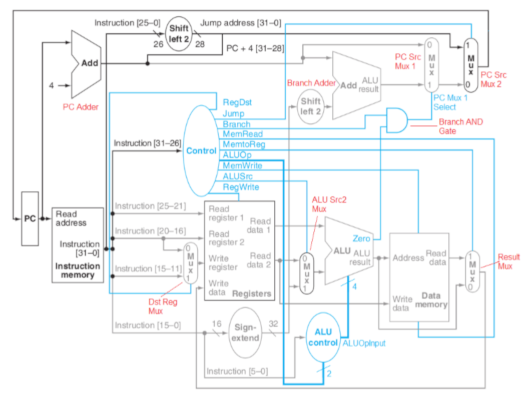
\includegraphics[scale=2]{datapath.png}
\caption{Datapath.}
\end{figure}
%\begin{figure*}[htbp]
%\centerline{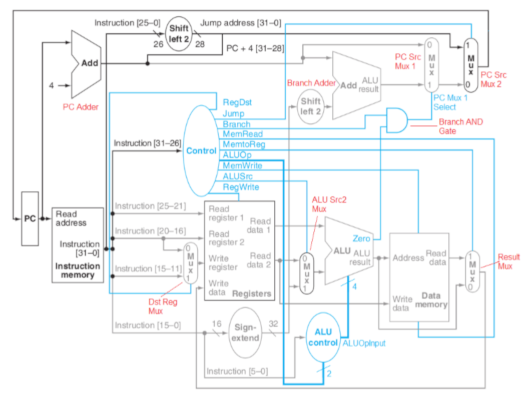
\includegraphics[scale=0.25]{datapath.png}}
%\caption{Datapath.}
%\label{fig_data}
%\end{figure*}

As we can see all the components are connected using wires.
\subsection{ModelSim}
We start developing our components in verilog, in order to maintenance and following the
standard principles of software developing  we create each module separatedly in its corresponding
.v file, e.g. regfile.v for the Register File component.
In total we have the following 17 files for all the modules:

\begin{table}[htbp]
\begin{center}
\begin{tabular}{c c}
\verb$regfile_lab5.v$&\verb$shift16_module.v$\\
\verb$alu_lab5.v$&\verb$instrumem.v$\\
\verb$extendbit_lab5.v$&\verb$ControlDataPath.v$\\
\verb$alucontrol.v$&\verb$mux31.v$\\
\verb$Select_word_half.v$&\verb$mux_5bits.v$\\
\verb$shift_left_2.v$&\verb$pccounter_4.v$\\
\verb$PC_module.v$&\verb$concatenar.v$\\
\verb$adder32.v$&\verb$complete_32bits.v$\\
\verb$proyecto_final.v$&\\
\end{tabular}
\end{center}
\end{table}

To clarify the terms every CPU component will be created in ModelSim as a module \cite{b4}.

\begin{figure}[htbp]
\centerline{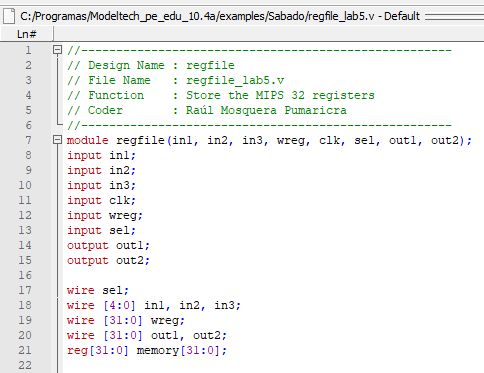
\includegraphics[scale=0.7]{modelsim_module.png}}
\caption{Register File module in ModelSim.}
\label{fig}
\end{figure}

\section{Experimental Setup} %III Experimental Setup
To test our datapath we first test each component separetly to isolate the
problems, once all the components pass its respective tests we continue with a complete 
test of our datapath, in order to do that we agroup the previous instructions
in 3 files to be loaded in the instruction memory.

Each test bench file contains the instructions and its respective
operands (registers). Previously for purpose testing we load the 
register file with random values.

\begin{table}[htbp]
\caption{Registers} %Testbench 1
\begin{center}
\begin{tabular}{|c|c|c|}
%\cline{2-4} 
\hline
Register&Number in decimal&Number in hexadecimal\\
number&notation&notation\\
\hline
16&49527&0000C177\\
\hline
17&63767&0000F917\\
\hline
18&31778&00007C22\\
\hline
19&23198&00005A9E\\
\hline
20&917&00000395\\
\hline
21&24182&00005E76\\
\hline
22&52687&0000CDCF\\
\hline
23&20726&000050F6\\
\hline
29&150&00000096\\
\hline
\multicolumn{3}{l}{The others registers, 1 to 15, 24 to 28 and 30,31 remain with zero.}
\end{tabular}
\label{tab_regfile}
\end{center}
\end{table}

In each test bench are using 10 nanoseconds as a positive clock signal and negative
clock signal which give us 20 nanoseconds in total per clock cycle.

\begin{table}[htbp]
\caption{Testbench 1} %Testbench 1
\begin{tabular}{|c|c|c|}
\hline
\multicolumn{3}{|c|}{\textbf{Instructions}} \\
%\cline{2-4} 
\hline
ADD&Subtraction (SUB)&AND  \\
\hline
NOR&OR&Set Less Than (SLT) \\
\hline
Add Immediate&Subtraction Inmediate & AND Inmediate \\
(ADDI) &(SUBI) & (ANDI) \\
\hline
OR Immediate&Set Less Than Immediate&  \\
(ORI)&(SLTI)&  \\
\hline
\end{tabular}
\label{tab_test1}
\end{table}

\begin{table}[t]
\caption{Testbench 2} %Testbench 2
\begin{center}
\begin{tabular}{|c|c|c|}
\hline
\multicolumn{3}{|c|}{\textbf{Instructions}} \\
%\cline{2-4} 
\hline
Store Byte&Store Halfword&Store Word\\
(SB)&(SH)&(SW)  \\
\hline
Load Byte&Load Halfword&Load Word\\
(LB)&(LH)&(LW) \\
\hline
Load Upper Inmediate&&\\
(LUI)&& \\
\hline
\end{tabular}
\label{tab_test2}
\end{center}
\end{table}

\begin{table}[htbp]
\caption{Testbench 3} %Testbench 3
\begin{center}
\begin{tabular}{|c|c|c|}
\hline
\multicolumn{3}{|c|}{\textbf{Instructions}} \\
%\cline{2-4} 
\hline
Branch On Equal&Branch On Not Equal&Branch On Greater \\
(BEQ)&(BNEQ)&than equal zero (BGEZ)  \\
\hline
Jump&Jump and Link&Jump Register\\
(J)&(JAL)&(JR) \\
\hline
\multicolumn{3}{l}{Since we need to simulate the branch and the jumps between the} \\
\multicolumn{3}{l}{instructions additional instructions were added i.e. ADDI and  SUB}\\
\end{tabular}
\label{tab_test3}
\end{center}
\end{table}

To get a real aproach of the use of the processor we will run the following C code.
\begin{figure}[h]
\begin{center}
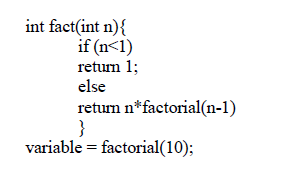
\includegraphics[scale=0.8]{factorial_c.png}
\caption{Factorial function - C code.}
\label{fact_c}
\end{center}
\end{figure}

The translation into MIPS instructions it would be as follow:
\begin{figure}[h]
\begin{center}
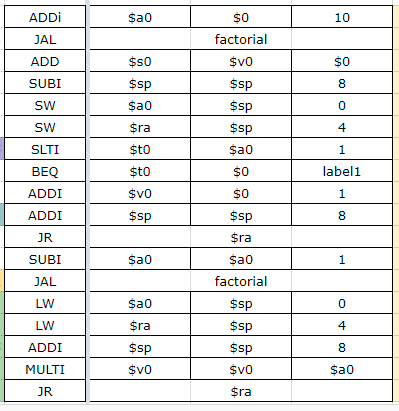
\includegraphics[scale=0.55]{factorial_mips.png}
\caption{Factorial function - MIPS.}
\label{fact_mips}
\end{center}
\end{figure}
 
As we can use the factorial function will use most of the intructions implemented and the recursivity
technique, this will be our test bench 4.

To calculate the CPU time \cite{b5} (time processing) for each test bench we use the following formula:
\[Time = PI * CPI * Time per Clock Cycle\] 

where PI is Program Instructions and CPI is Clock Cycles per instruction. 

\begin{table}[h]
\caption{Clock cycles} %Clock cycles
\begin{center}
\begin{tabular}{|c|c|c|c|c|}
\hline
&Total&Total executed&Clock&CPU Time\\
&instructions&instructions&Cycles&(Nanoseconds)\\
&&(Expected)&&\\
\hline
Test bench 1&11&11&11&220\\
\hline
Test bench 2&7&7&7&140\\
\hline
Test bench 3&22&17&17&340\\
\hline
Test bench 4&18&131&131&2620\\
\hline
\end{tabular}
\label{tab_test3}
\end{center}
\end{table}

%EVALUATION SECTION
\section{Evaluation}
We executed the test bench 1, 2, 3 and 4, these were the results:

\begin{figure}[h]
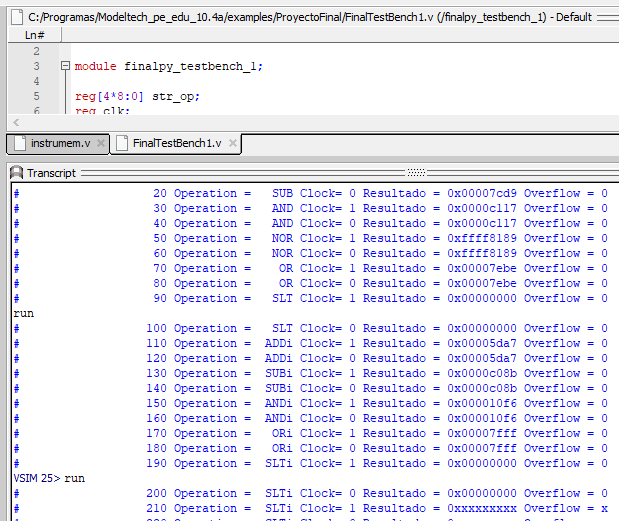
\includegraphics[scale=0.41]{ModelSim_testbench1_clock_cycles.png}
\caption{Execution results for test bench 1.}
\label{result1}
\end{figure}

We ran the test bench in intervals of 100 nanoseconds as we can see in Fig. 5. \label{result1}. For the 
test bench 1 we get 100 nanoseconds + 100 nanoseconds + 20 nanoseconds with in total 
give us 220 nanoseconds.

We apply the same procedure to the test bench 2  \label{result3}, Fig. 8. and the result was
100 nanoseconds + 40 nanoseconds = 140 nanoseconds.

In test bench 3, Fig. 9., we got 100 nanoseconds + 100 nanoseconds + 100 nanoseconds 
+ 40 nanoseconds with th total of 340 nanoseconds.

And finally for the test bench 4, Fig. 6, we use intervals of 500 nanoseconds since the execution
is elevated, we get 2610 nanoseconds in total also the output of the factorial of 10 was 
0x003750f00 which in decimal notation correspond to 3628800.

\begin{figure}[h]
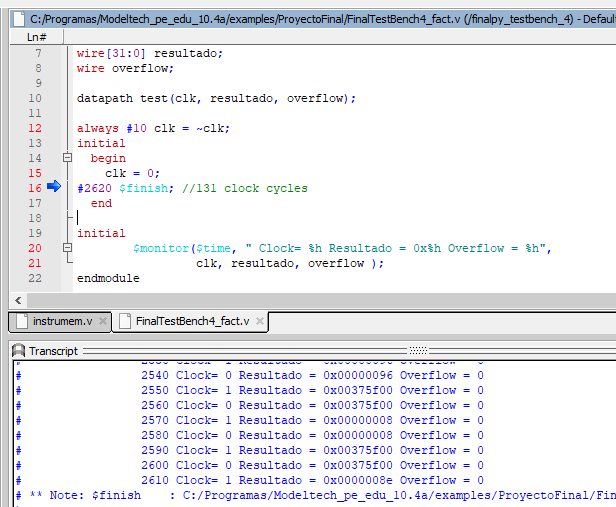
\includegraphics[scale=0.5]{ModelSim_factorial4_clock_cycles.png}
\caption{Execution results of the test bench for the factorial.}
\label{result_factorial}
\end{figure}

\begin{figure}[h]
\begin{center}
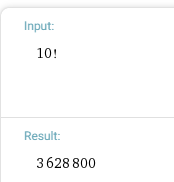
\includegraphics[scale=0.7]{factorial_10.png}
\caption{Wolfram Alpha - Factorial of 10. \cite{b6}}
\label{result_factorial}
\end{center}
\end{figure}

\begin{figure}[h]
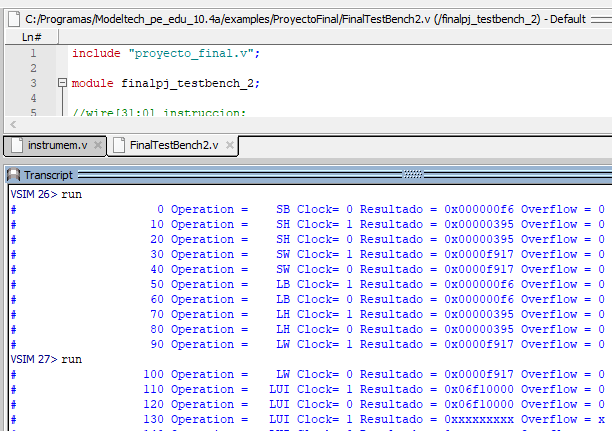
\includegraphics[scale=0.5]{ModelSim_testbench2_clock_cycles.png}
\caption{Execution results for test bench 2.}
\label{result2}
\end{figure}

\begin{figure}[h]
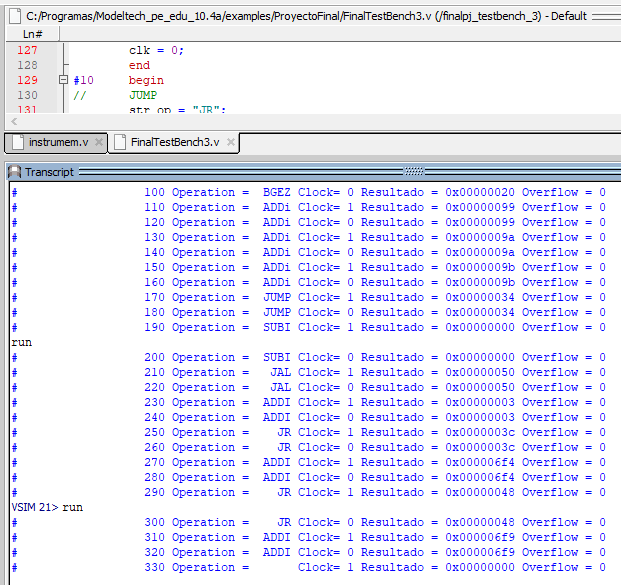
\includegraphics[scale=0.5]{ModelSim_testbench3_clock_cycles.png}
\caption{Execution results for test bench 3.}
\label{result3}
\end{figure}

Comparing the results of Fig. 5., Fig. 8. and Fig. 9. with the Table VIII we get the same amount
of clock cycles and the time for each file, also the results of the instructions are as we expected.
 
%CONCLUSION SECTION
\section{Conclusion}
\begin{itemize}
\item Since the single cycle datapath was the original solution in the early days of RISC architecture nowadays
is not efficient because it takes 1 cycle per instruction when another aproachs using the pipeline technique
could reduce the cycle needed per instruction. 
\item It became mandatory calculate the expected time processing for test our datapath, otherwise we could
get unexpected result since the execution continue with the next instruction, like for example in our test bench
for the factorial.
\item Before start coding in ModelSim we need to decide if we are going to apply the clock edge 
triggered and which modules will apply for that, because if not the major changes needed 
in the modules would be very risky and will take more time for testing.
\item Verilog was not specially designed to upload files that why for our tests purposes we need to
modify the code to point a specific file. 
\end{itemize}
%COMMENTS SECTION
\section{Comments}
\begin{itemize}
\item When we are simulating our component in ModelSim no warnings must appear when the 
simulation starts, otherwise there was some error or unexpected behaviour. One common 
issue is referring a wire or register as an input or output of a module with diferent length.
\item In ModelSim is the identifier is not declare verilog assume is a wire.
\item The verilog compiler doesn't warn you when a module  instantiation does not exists until you simulate it
\item One common problem is asume the execution of the code in the components of the datapth will be sequential, 
that is not correct since we have the always @ block and that could be executed in the upper sign of the clock 
or the lower sign.
\item For those who are used to the conditional statements of the programming languages it is a little difficult at the 
beginning use verilog, because at the digital circuit level there we only have and, or, xor and all the gates.
\item To find the errors in the testing fase we can navigate in the windows objects in ModelSim throught the modules
to find the issue.
\end{itemize}

\begin{thebibliography}{00}
\bibitem{b1} MIPS.com. (2016). MIPS® Architecture for Programmers Volume II-A: The MIPS32® Instruction Set Manual. [online] Available at: \url{https://s3-eu-west-1.amazonaws.com/downloads-mips/documents/MD00086-2B-MIPS32BIS-AFP-6.06.pdf} [Accessed 27 Nov. 2018].
\bibitem{b2} IEEE Standard for Verilog Hardware Description Language. IEEE Standard 1364-2005 (Revision of IEEE Standard 1364-2001). \url{http://dx.doi.org/10.1109/IEEESTD.2006.99495}, 2006. Last access 26 November 2018.
\bibitem{b3} Mentor.com. (2018). ModelSim PE Student Edition. [online] Available at: \url{https://www.mentor.com/company/higher_ed/modelsim-student-edition} [Accessed 27 Nov. 2018].
\bibitem{b4} Ashenden, P. (2008). Digital Design: An Embedded Systems Approach Using Verilog. Burlington, MA: Elsevier Science, pp.22,23.
\bibitem{b5} Patterson, D., Hennessy, J. and Alexander, P. (2012). Computer organization and design. 4th ed. Waltham, Mass: Morgan Kaufmann, pp.35.
\bibitem{b6} Wolframalpha.com (2018). Wolfram|Alpha: Making the world’s knowledge computable. [online] Wolframalpha.com. \url{Available at: https://www.wolframalpha.com/input/?i=factorial+10} [Accessed 28 Nov. 2018].
\end{thebibliography}
\vspace{12pt}

\end{document}
